\appendix

\INEchaptercarta{Aspectos metodológicos}{}

$\ $\\[-2cm]
\titulo{Diseño muestral de la Encovi}

El esquema de muestreo adoptado para la ENCOVI 2014 es de tipo probabilístico, bietápico, estratificado y por conglomerados, donde la unidad última de selección está constituida por doce viviendas ocupadas, seleccionadas con igual probabilidad al interior de cada unidad primaria de muestreo (UPM). Cada UPM fue seleccionada de manera sistemática y proporcional al tamaño (PPT), con afijación proporcional en las áreas urbanas y rurales y al interior de ellas en 4 estratos urbanos y 4 rurales.

\begin{itemize}
	\itemsep 16pt
	\item [\large\textbf{a)}$\ $]	\textbf{\large Dominios de estudio  y cobertura: }\\[3mm]
	El diseño muestral contempla para sus estimaciones y proceso inferencial 22 dominios de estudio, los cuales son independientes y mutuamente excluyentes. Los dominios de estudio lo comprenden los 22 departamentos de la República, pudiendo integrarse por región, total país urbano, total país rural y total del país. La cobertura de la encuesta es entonces nacional y abarca la división político-administrativa del país.
	
	
	
	\item[\large\textbf{b)}$\ $]	\textbf{\large Marco muestral y selección de la muestra:} \\[3mm]
	El marco muestral total de la ENCOVI es el Marco Maestro de Muestreo (MMM) o Marco Nacional, el cual está constituido por 15,511 Unidades Primarias de Muestreo (UPM) o sectores cartográficos, equivalentes a 2,127,915 viviendas ocupadas, con un promedio burdo general de 137.19 viviendas por UPM.
	
	Este MMM fue elaborado con base a los datos de los Censos de  Población y Vivienda de 2002,  estratificado atendiendo el nivel socioeconómico en función de variables como  las Necesidades Básicas Insatisfechas (NBI), el nivel educativo del jefe de hogar y otras relacionadas con el nivel socio-económico, utilizando para ellos el algoritmo multivariado de las “k” medias. 
	
	Esta estratificación produjo como resultado final 8 estratos por departamento, de los cuales 4 son urbanos y 4 rurales; el Marco Maestro de Muestreo (MMM) comprende, entonces, 176 estratos distribuidos en los 22 departamentos y dos áreas o ámbitos cada uno. 
	
	Del marco, se calculó y seleccionó  de manera sistemática y  con probabilidades proporcionales al tamaño (PPT) una Muestra Maestra (MM) cuyo tamaño es de 4,116 UPM, equivalentes a 621,172 viviendas ocupadas. Esta muestra maestra fue diseñada para utilizarla como marco de selección para encuestas de hogares a  partir del 2008.
	
	La selección de las UPM de la ENCOVI se realizó también de manera sistemática y con PPT de la Muestra Maestra (MM) se seleccionaron 1,037 sectores cartográficos como muestra de primera etapa.
	
	El marco muestral de segunda etapa para la ENCOVI lo constituye la actualización cartográfica (trabajo de mapeo) la cual genera una lista de $n$ viviendas ocupadas para cada una de las 1,037 UPM de la muestra de primera etapa. En cada uno de estas 1,037 listas de las $n$ viviendas ocupadas se construyen segmentos compactos de 6 viviendas cada uno, seleccionándose 2 con igual probabilidad por cada UPM, es decir una muestra total de segunda etapa de 2,074 unidades secundarias de muestreo (USM). 
	
	\item[\large\textbf{c)}$\ $]	\textbf{\large El tamaño de la muestra y su distribución:} \\[3mm]
	Para la ENCOVI 2014 el tamaño total de muestra se obtiene integrando los tamaños de muestra de cada uno de los 22 dominios de estudio y es de 1,037 sectores cartográficos (UPM) que representa aproximadamente 12,444 viviendas. 
	
	Para determinar el tamaño de muestra, en los cálculos se asume un valor de efecto de diseño (DEFF), una precisión relativa esperada para la variable principal, una tasa de no respuesta en base a encuestas anteriores, la tasa de pobreza extrema (variable principal), el promedio de personas por hogar, el error máximo relativo esperado y un nivel de confiabilidad adecuado (valor z de una distribución normal de probabilidades). El algoritmo utilizado para el cálculo de la muestra (en hogares) fue el siguiente:
	
	\begin{center}
		$n=\dfrac{Z^2(1-p)\text{\textsc{DEFF}}}{e^2p(1-\text{\textsc{TNR}})\bar{X}}$,
	\end{center}
	
	
	donde $Z $ es el valor de una distribución normal de probabilidad correspondiente  al nivel de confiabilidad asumido (95\%), siendo este igual a 1.96; $\ p $ es la proporción considerada en la variable principal (Tasa de Pobreza Extrema); $\ DEFF $ es el efecto de diseño,  que es la pérdida o ganancia en la eficiencia del diseño por efecto de estratificación y/o  conglomerar elementos de la población, para formar unidades muestrales, se obtiene del cociente entre la varianza de la variable en el  diseño complejo y la varianza de la variable, considerando un muestreo aleatorio simple; $\ e $ es el error relativo máximo esperado; $\ TNR $ es la tasa de no respuesta o porcentaje de rechazo; $\ \bar{X}$ es el promedio personas por hogar.
	
	
	El algoritmo que se aplicó para cada uno de los 22 dominios, permitió obtener así: 22 muestras independientes y excluyentes; estas muestras se afijaron proporcionalmente a los ámbitos urbano y rural y a los estratos dentro de cada domino y área. 
	
	Para realizar la selección de UPM fue necesario convertir la muestra en hogares a viviendas y luego la muestra de viviendas a sectores cartográficos. Para tal efecto se utilizó la estructura del marco maestro en viviendas y hogares, a nivel de estrato, área y departamento. El siguiente cuadro resumen permite apreciar la muestra total y su distribución en los 22 dominios y los ámbitos urbano y rural:
		
	$\,$\\[-0.7cm]
	\begin{center}
		\begin{tabular}{lcc}
			\hline &&\\[-0.56cm]
			\multicolumn{1}{c}{\multirow{2}[0]{*}{\textbf{Departamento}}}  & \multirow{2}[0]{*}{\textbf{Sectores}} & \multirow{2}[0]{*}{\textbf{Vivienda}} \\[0.22cm]
			\hline
			&&\\[-0.34cm]
			
			\textbf{Total general}	&	\textbf{1037}	&	\textbf{12444}	\\
			Guatemala	&	90	&	1080	\\
			El Progreso	&	43	&	516	\\
			Sacatepéquez	&	75	&	900	\\
			Chimaltenango	&	50	&	600	\\
			Escuintla	&	67	&	804	\\
			Santa Rosa	&	36	&	432	\\
			Sololá	&	40	&	480	\\
			Totonicapán	&	40	&	480	\\
			Quezaltenango	&	65	&	780	\\
			Suchitepéquez	&	54	&	648	\\
			Retalhuleu	&	36	&	432	\\
			San Marcos	&	40	&	480	\\
			Huehuetenango	&	40	&	480	\\
			Quiché	&	40	&	480	\\
			Baja Verapaz	&	32	&	384	\\
			Alta Verapaz 	&	35	&	420	\\
			Petén	&	50	&	600	\\
			Izabal	&	35	&	420	\\
			Zacapa	&	33	&	396	\\
			Chiquimula	&	33	&	396	\\
			Jalapa	&	43	&	516	\\
			Jutiapa	&	60	&	720	\\[0.05cm]
			\hline
		\end{tabular}
	\end{center}
	
	
	
	Los parámetros  considerados para el cálculo de estos tamaños de muestra fueron los siguientes: Un nivel de confiabilidad del 95\%; un efecto de diseño de 2, tomado del promedio de las estimaciones para distintas variables efectuadas en la ENCOVI-2006; asimismo, se asumió un error máximo relativo esperado del 12\% para la estimación de la tasa de pobreza extrema, los promedios de personas por hogar para cada departamento fueron estimados con la información de la ENCOVI-2006; la tasa de no respuesta se fijó en 10\% para todos los departamentos excluyendo el de Guatemala donde se asumió 15\% en base a experiencias previas.
	
	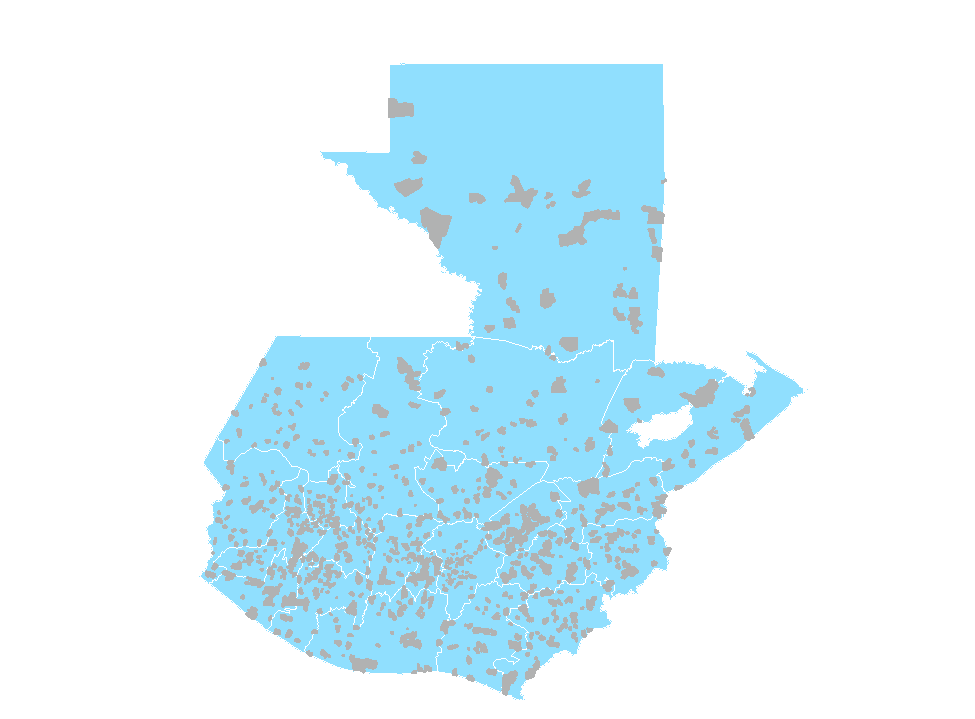
\includepdf{mapa1.pdf}	
	
	\item[\large\textbf{d)}$\ $]	\textbf{\large Validez inferencial, expansores y niveles de desagregación de resultados:} \\[3mm]	
	
	La validez inferencial de la muestra de ENCOVI-2014 para la variable principal que es la tasa de pobreza extrema, está garantizada con un nivel de confiabilidad del 95\%, un error relativo esperado de alrededor del 12\% y un efecto de diseño de 2, parámetros asumidos en el cálculo del tamaño de las muestras de los dominios de estudio. 
	
	Para el resto de las variables indagadas se esperan parámetros cercanos  a estos, y es evidente que  cuanto menos se relacione cierta variable con la variable principal su precisión relativa, error estándar de estimación e intervalos de confianza serán  menos precisos o más lejanos a los asumidos. 
	
	Los factores de expansión serán calibrados con proyecciones de población al momento de la encuesta y ajustados y calculados con cuatro componentes: 1) el ajuste por no respuesta, 2) la expansión de USM a UPM, 3) la expansión a la Muestra Maestra y, 4) la expansión de la Muestra Maestra al Marco Maestro. Estos actúan expandiendo hasta un estrato dentro de un sector, las referidas expansiones se integran a todo el ámbito (urbano, rural), luego se integran a nivel del dominio (departamento), y continúan a región (si se desea) y finalmente a nivel nacional (todo el país).
	
	La desagregación de resultados conforme al diseño es válida y garantiza los parámetros inferenciales a los siguientes niveles:
	
	
	\begin{itemize}
		\item Todo el país
		\item Todo el país urbano
		\item Todo el país rural
		\item Toda una región
		\item Todo un departamento 
		
	\end{itemize}
	
	Estos niveles de desagregación, son aplicables a todas las variables que indaga la encuesta, indicando que los intervalos de confianza serán más amplios para todas aquellas variables “lejanas” o poco correlacionadas con la variable principal del diseño, asimismo las estimaciones serán menos precisas y los errores  de estimación mayores.
	
	
\end{itemize}


